\scanpage{7}
\mspage{5}

\figure{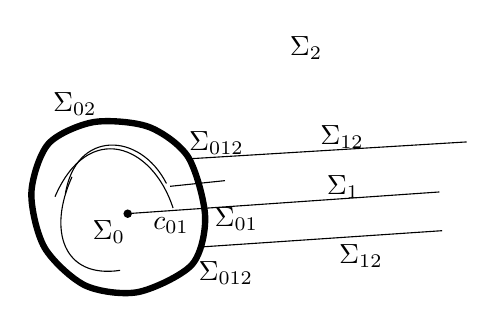
\begin{tikzpicture}[x=0.012cm,y=-0.012cm]
\draw[line width=2.3pt] plot[smooth cycle] coordinates {(267,310) (285,258) (333,235) (391,240) (433,272) (451,335) (437,386) (380,415) (324,408) (281,368)};
\draw (303,311) .. controls (314,243) and (382,245) .. (410,300);
\draw (292,314) .. controls (327,233) and (395,258) .. (417,326);
\draw (310,293) .. controls (284,350) and (301,401) .. (361,392);
\draw (414,303)--(472,297) (432,274)--(728,256) (368,332)--(699,309) (450,367)--(702,350);
\fill (369,332) circle (4.5);
\node at (558,157) {$\Sigma_2$};\node at (313,216) {$\Sigma_{02}$};
\node at (463,257) {$\unsure{\Sigma_{012}}$};\node at (596,251) {$\Sigma_{12}$};
\node at (349,351) {$\Sigma_0$};\node at (415,345) {$\unsure{c_{01}}$};
\node at (484,338) {$\Sigma_{01}$};\node at (597,304) {$\Sigma_1$};
\node at (473,395) {$\Sigma_{012}$};\node at (616,377) {$\Sigma_{12}$};
\end{tikzpicture}}
\margin{$\unsure{3}\quad\unsure{\uparrow}$}

\figure{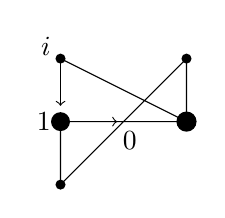
\begin{tikzpicture}[x=0.8cm,y=0.8cm]
\draw (0,2)--(2,1)--(2,2)--(0,0)--(0,1)--(2,1);
\draw[->] (0,2)--(0,1.25);\draw[->] (0,1)--(0.9,1);
\foreach \x/\y in {0/0,0/2,2/2}{\fill (\x,\y) circle (0.08);}
\fill (0,1) circle (0.15);\fill (2,1) circle (0.16);
\node[left] at (0,2.2) {$\unsure{i}$};\node[left] at (0,1) {$1$};\node[below] at (1.1,1) {$0$};
\end{tikzpicture}}

$\Sigma_{i_0i_1\ldots i_n}$\qquad\deleted{\unsure{covariant}} foncteur contravariant
par rapport aux drapeaux
variables $(i_0,\ldots,i_n)$
\[
\Sigma_i=X_i'=X_i\setminus\left(X_i\cap\bigcup_{k<i}\unsure{\mathring{\operatorname{Tub}}}(X_k,X_i)\right)
\]
\[
\Sigma_{(i,j)}=\deleted{\unsure{\partial}}\operatorname{Tub}^{\unsure{\bullet|\circ}}
\left(X_i',X_j\deleted{\unsure{\varnothing}}\setminus
\bigcup_{\substack{\deleted{\unsure{k<j}}\\\deleted{\unsure{k\ne i}}\\\inserted{i<k<j}}}
\operatorname{Tub}(X_k,X_j)\right)\hookrightarrow X_j'=\Sigma_j
\]
\[
i<k<j
\]

\margin{\diagram{\begin{tikzcd}
\Sigma_\delta\arrow[r,hook]\arrow[d]&\Sigma_{\delta'}\arrow[d]\\
\Sigma_d\arrow[r,hook]&\Sigma_{d'}
\end{tikzcd}}
\diagram{\[\begin{array}{ccc}d&\supset&d'\\\cap&&\cap\\\delta&&\delta'\end{array}\]}
cofinaux
\diagram{\begin{tikzcd}\unsure{\bullet}\arrow[d]\\d'\end{tikzcd}}}

\deleted{$\Sigma_{i,j}=F$}
\diagram{\begin{tikzcd}[column sep=large]
\mathcal V_{ij}=\mathcal V(X_i^*,X_j)\setminus\displaystyle\bigcup_{i\leq k<j}\mathcal V(\unsure{X_i^*|X_i'},X_j)\cap X_k\arrow[r,hook]\arrow[d]&X_j^*\\
X_i^*&
\end{tikzcd}}
\[
X\qquad\mathcal V_{ijk}
\]
\diagram{\begin{tikzcd}[row sep=large,column sep=large]
\mathcal V_{ijk}\arrow[r]\arrow[d]&\mathcal V_{jk}\arrow[d]&X_k^*\arrow[l,hook]\arrow[d,"\unsure{\sim}"']\\
\mathcal V_{ij}\arrow[r,hook]\arrow[d]&\mathcal V(X_j^*,X_k)\arrow[r,"\deleted{\unsure{\sim}}"]&\deleted{X_k}\\
X_i^*&&
\end{tikzcd}}

\margin{$\lambda_i'T'=\lambda_i''T''$\qquad
$a\leq\operatorname{Inf}(\lambda_i',\lambda_i'')$}
\margin{6}
